\section*{Приложение}
\addcontentsline{toc}{section}{Приложение}
\label{sec:Appendix}

\subsection*{Дополнительные результаты работы модели, вдохновлённой CFRWD-GAN}

\begin{figure}[H]
    \centering
    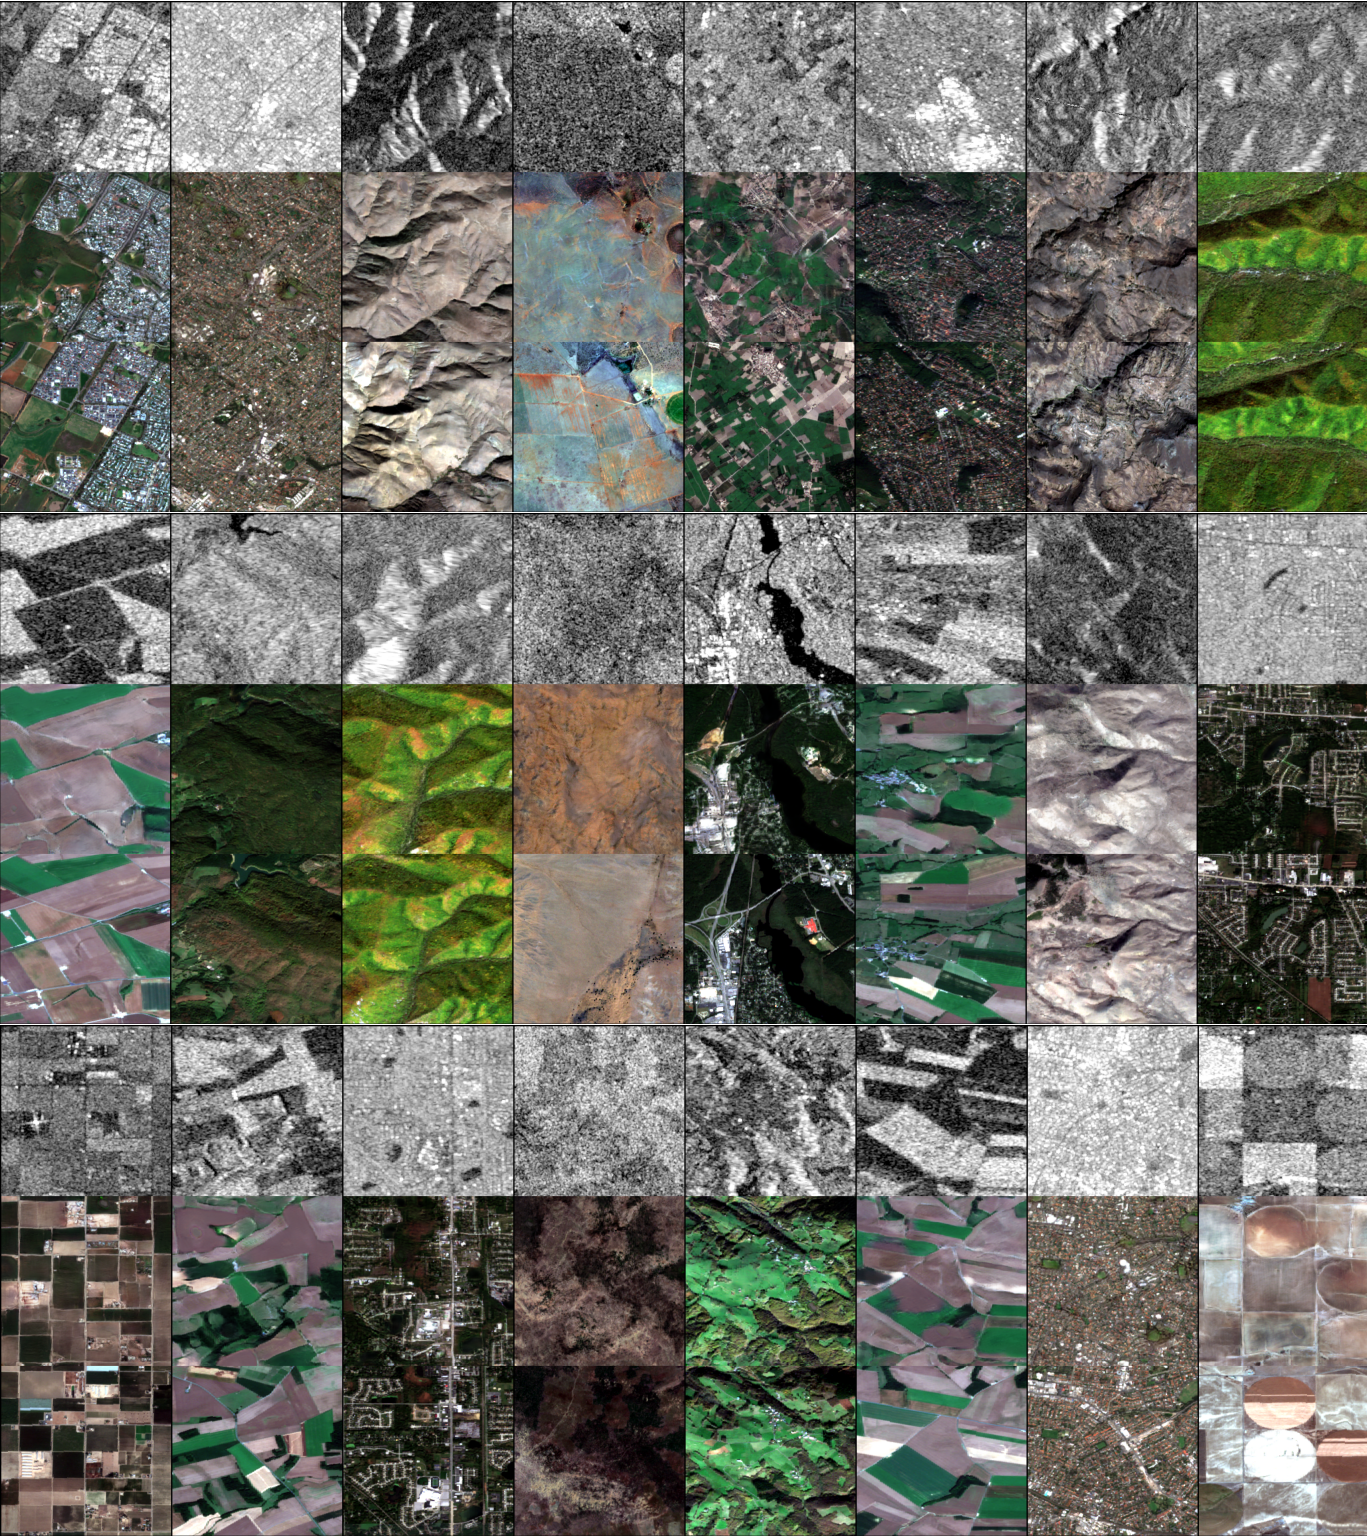
\includegraphics[width=0.95\linewidth]{images/cfrwd/output/val/val_figures_1-3.png}
    \caption{Примеры трансляции SAR-изображений. Строки сверху вниз: (а) входное радиолокационное изображение; (б) результат генерации модифицированной модели; (в) целевое оптическое изображение (ground truth).}
    \label{fig:appendix_cfrwd_val_figures_1-3}
\end{figure}

\begin{figure}[H]
    \centering
    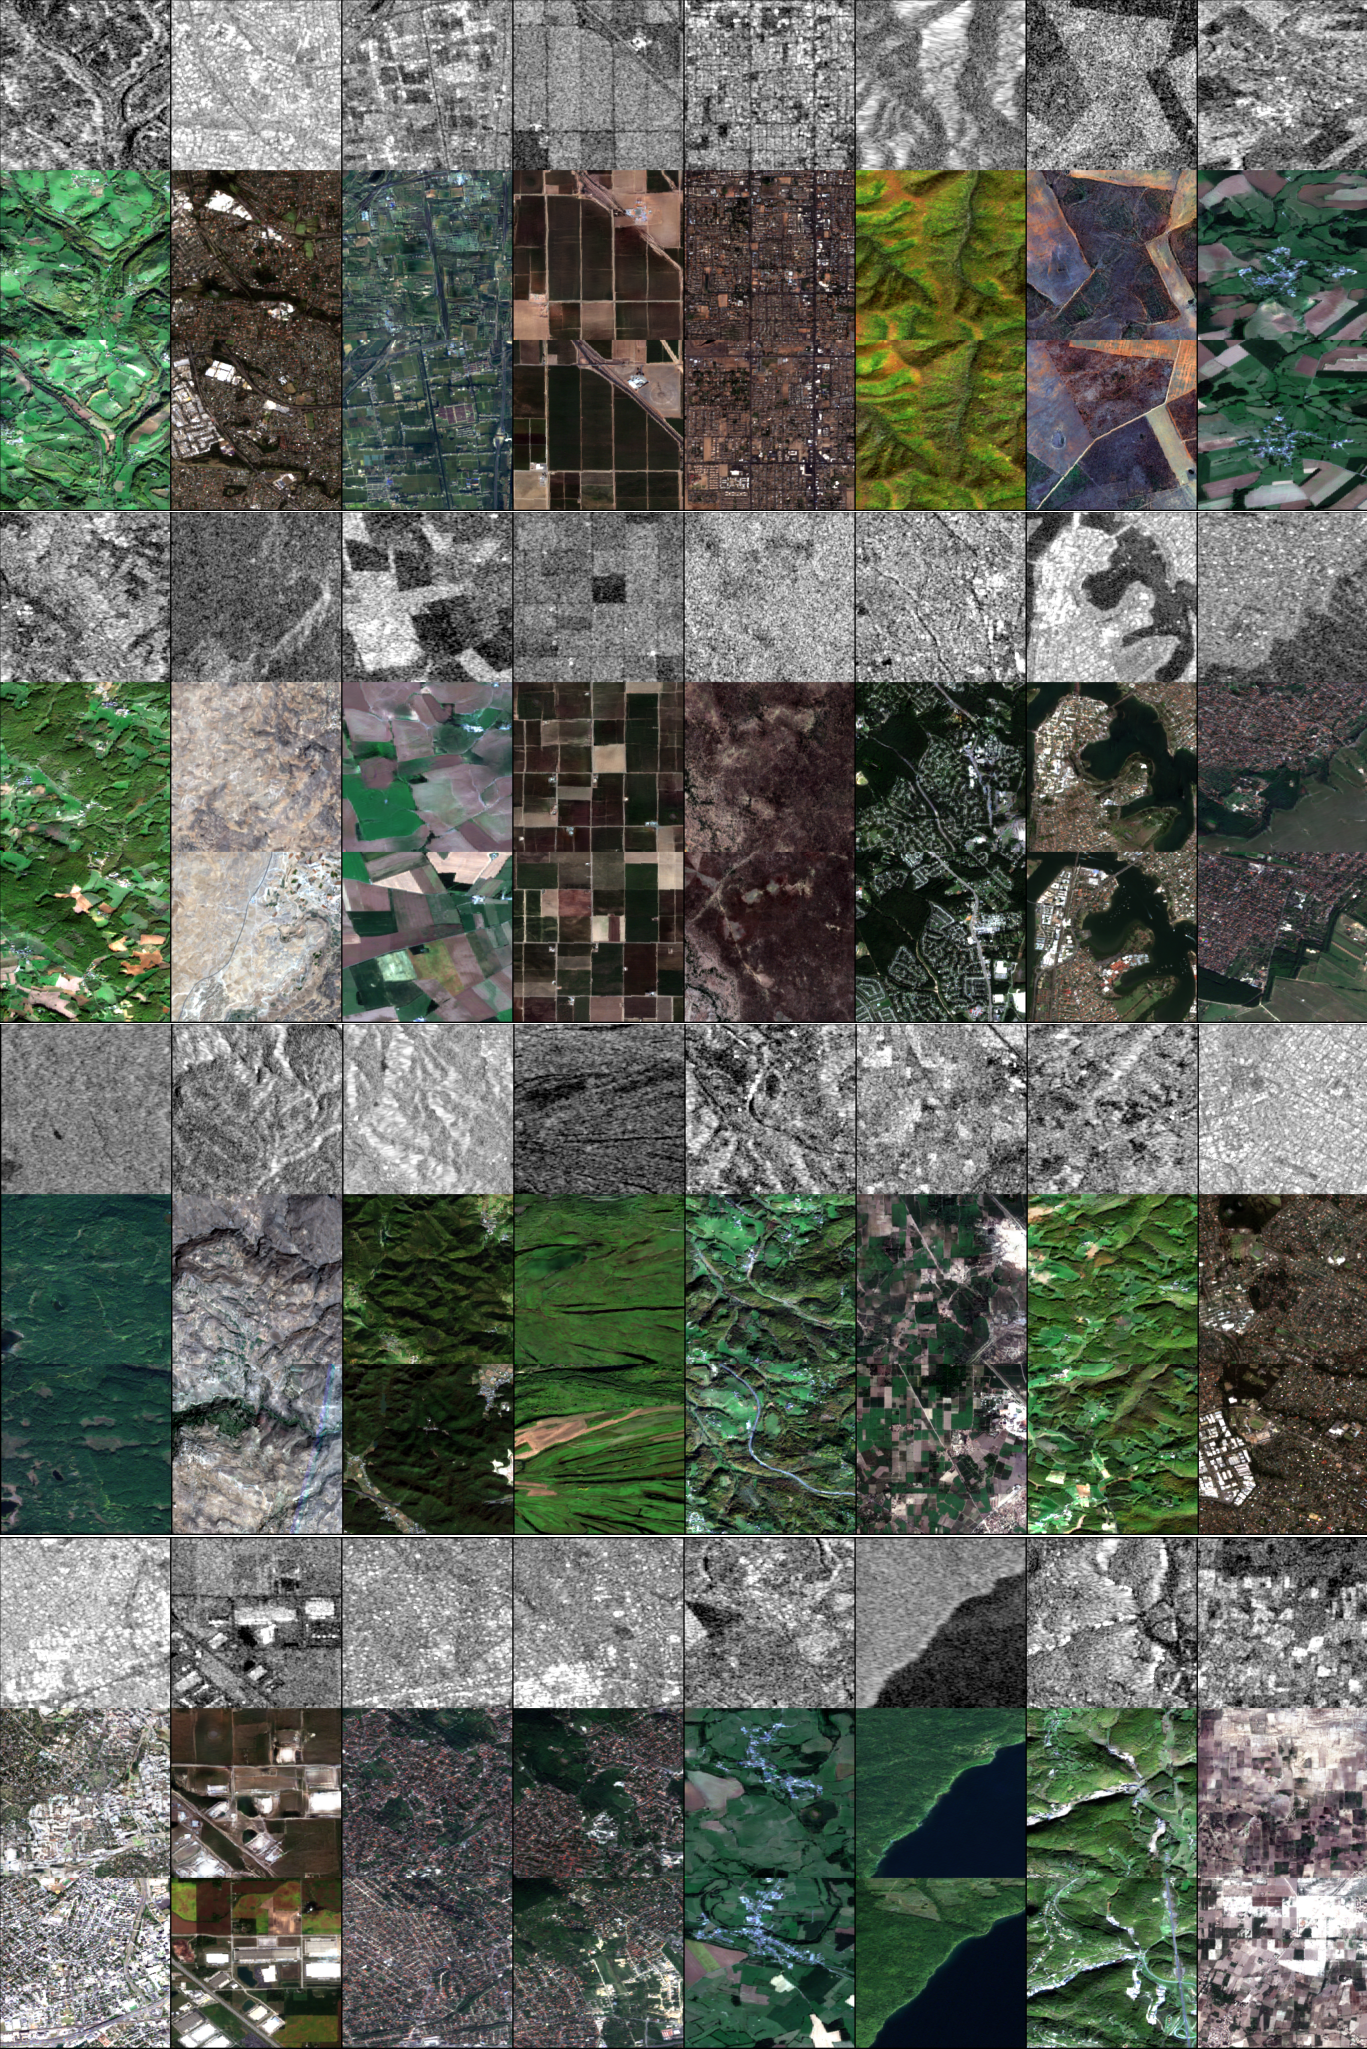
\includegraphics[width=0.95\linewidth]{images/cfrwd/output/val/val_figures_4-7.png}
    \caption{Примеры трансляции SAR-изображений. Обозначения идентичны рис.~\ref{fig:appendix_cfrwd_val_figures_1-3}.}
    \label{fig:appendix_cfrwd_val_figures_4-7}
\end{figure}

\subsection*{Дополнительные результаты работы LLW-Former}

\newcommand{\llwpair}[4]{%
  \begin{figure}[H]
    \centering
    \begin{subfigure}[t]{0.48\linewidth}
      \centering
      \includegraphics[width=\linewidth]{images/llwt/output/#1.pdf}
      \caption{}\label{#2}
    \end{subfigure}\hfill
    \begin{subfigure}[t]{0.48\linewidth}
      \centering
      \includegraphics[width=\linewidth]{images/llwt/output/#3.pdf}
      \caption{}\label{#4}
    \end{subfigure}
    \caption{Примеры трансляции SAR-изображений. Слева SAR, посередине сгенерированное псевдооптическое изображение, справа целевое.}
  \end{figure}%
}

\llwpair{llw_scene_5}{fig:appendix_llw_scene_5}{llw_scene_52}{fig:appendix_llw_scene_52}
\llwpair{llw_scene_84}{fig:appendix_llw_scene_84}{llw_scene_100}{fig:appendix_llw_scene_100}
\llwpair{bad_llw_mountains}{fig:appendix_bad_llw_mountains}{bad_llw_urban}{fig:appendix_bad_llw_urban}